\section{Detection and Recognition Using Image Processing}
\setcounter{figure}{0}
\renewcommand{\thefigure}{5.\arabic{figure}}

In this Chapter, we will go through the full process of turning a single sided Braille page loaded with multiple characters and full of Braille dots that has been preprocessed into multiple arrays of zeros and ones representing all of the symbols in the page. This page has already been filtered and adjusted to be correctly oriented. 

Before going through the details, let's discuss the keywords used in this chapter. The term "Detection" refers to the process of locating each braille symbols in a page. Producing an output array that contains all of the locations of the dots in the page. On the other hand, the term "Recognition" refers to the process of identification of each symbol as a combination of 6 dots.

It is important before explaining the algorithm used for detection to mention the restriction to the input page. For simplicity we assumed that the input page would have multiple lines - full of symbols - and not just a line or two. This is to ensure a maximum accuracy in the detection process. The explanation for this restriction is to be discussed later in this chapter.
\subsection{Detection}
In this section we will discuss the methods used to extract locations of the dots in our Braille page. The two methods are mainly \textit{Canny Edge Detection} and \textit{Hough Circle Detection} which are complementary to each other.
\subsubsection{Edge Detection with Canny Algorithm}
Canny edge detection is a technique designed to extract essential structural details from various visual objects while significantly reducing the data that needs processing. It's widely used in different computer vision applications due to its effectiveness in meeting the general requirements for edge detection across diverse systems. These requirements include:
\begin{enumerate}
        \item Detecting edges with a low error rate to ensure that as many edges as possible in the image are accurately identified.
        \item Precisely localizing the detected edge points to the center of the edges.
        \item Ensuring that each edge in the image is marked only once and minimizing the impact of image noise to avoid false edges.
\end{enumerate}


To meet these criteria, Canny employed the calculus of variations, a technique that finds the function optimizing a given functional. The optimal function in the Canny detector is represented by the sum of four exponential terms but can be approximated by the first derivative of a Gaussian.

The Canny edge detection algorithm is one of the most well-defined methods for edge detection, known for its reliability and effectiveness. Due to its optimality in meeting the three key criteria and the simplicity of its implementation, it has become a popular choice for edge detection.

The Canny edge detection process involves five main steps:

\begin{enumerate}
        \item Apply a Gaussian filter to smooth the image and reduce noise. Fig.\ref{fig:num1}(b)
        \item Calculate the intensity gradients of the image. Fig.\ref{fig:num1}(c)
        \item Use gradient magnitude thresholding or lower bound cut-off suppression to eliminate spurious edge detection responses. Fig.\ref{fig:num1}(d)
        \item Apply a double threshold to identify potential edges. Fig.\ref{fig:num1}(e)
        \item Use edge tracking by hysteresis to finalize edge detection by suppressing weak edges that are not connected to strong edges. Fig.\ref{fig:num1}(f)
\end{enumerate}

\begin{figure}[H]
\centering
\subfloat[Original Image]{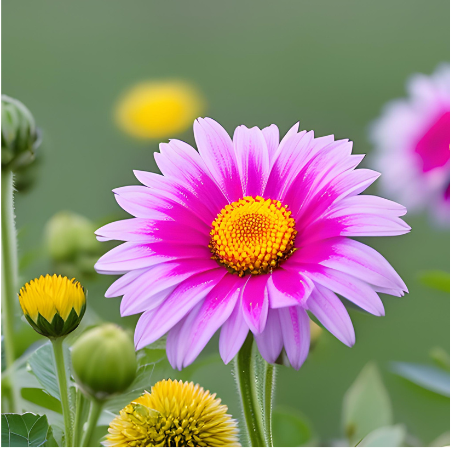
\includegraphics[width=0.45\linewidth]{Canny/0.png}}\hfill
\subfloat[Image after greyscale and noise reduction]{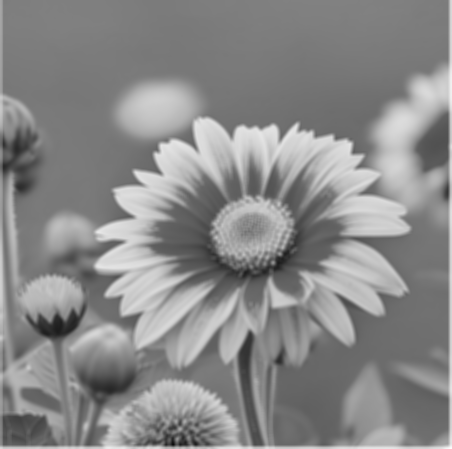
\includegraphics[width=0.45\linewidth]{Canny/1.png}}\\
\subfloat[After gradient calculation]{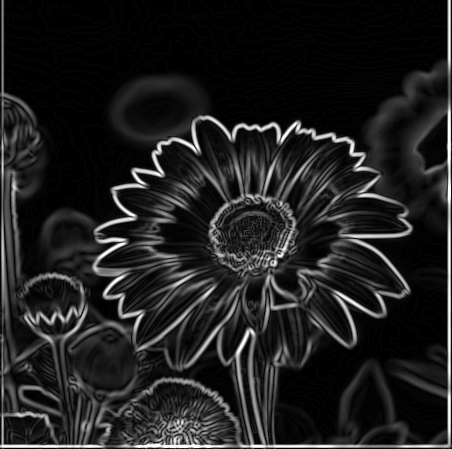
\includegraphics[width=0.45\linewidth]{Canny/2.png}}\hfill
\subfloat[After non-maximum suppression]{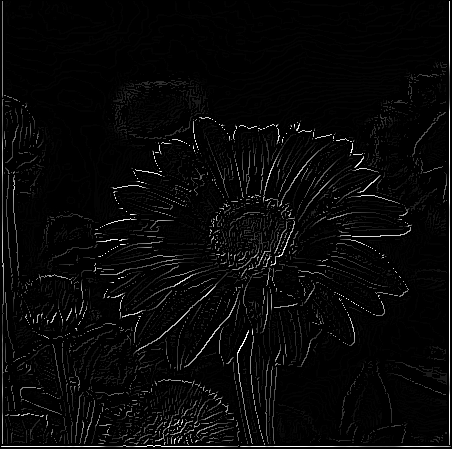
\includegraphics[width=0.45\linewidth]{Canny/3.png}}\\
\subfloat[Strong edges after double thresholding]{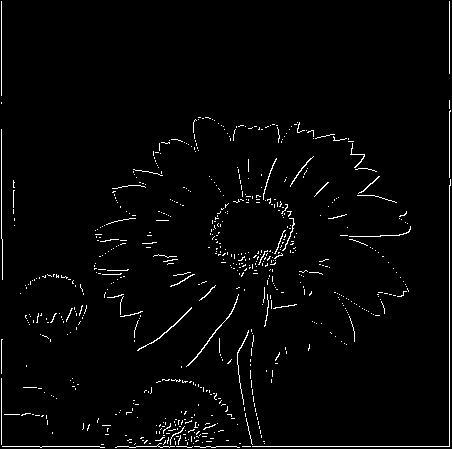
\includegraphics[width=0.45\linewidth]{Canny/4.png}}\hfill
\subfloat[Final edge tracking]{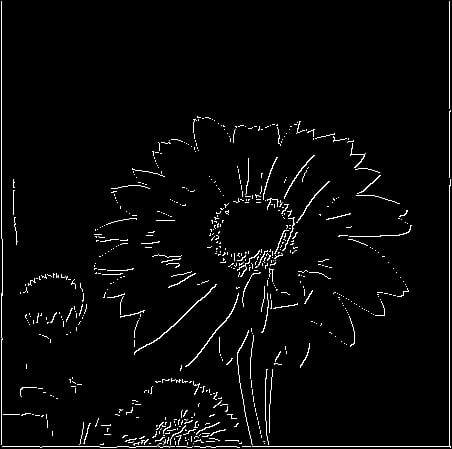
\includegraphics[width=0.45\linewidth]{Canny/5.jpeg}}
\caption{Canny Edge Detection Process}
\label{fig:num1}
\end{figure}
\clearpage

While dealing with a loaded page of Braille symbols, the process is just the same as mentioned above. All the manipulation is done through adjusting the parameters and resolution of the filters until getting the perfect output. Fig.5.2(b) shows the single sided Braille page after being processed with canny algorithm.
\begin{figure}[H]
    \centering
    \subfloat[Original Page (After Preprocessing)]{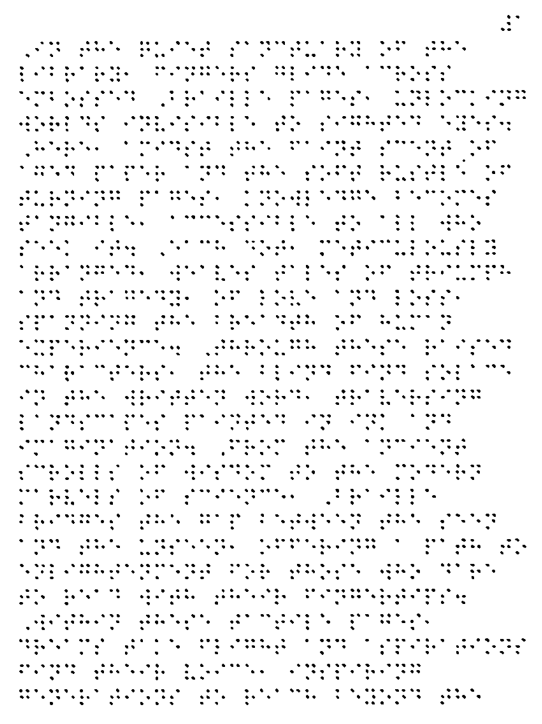
\includegraphics[width=0.5\linewidth]{Canny/filtered.png}}\hfill
    \subfloat[Detected Edges]{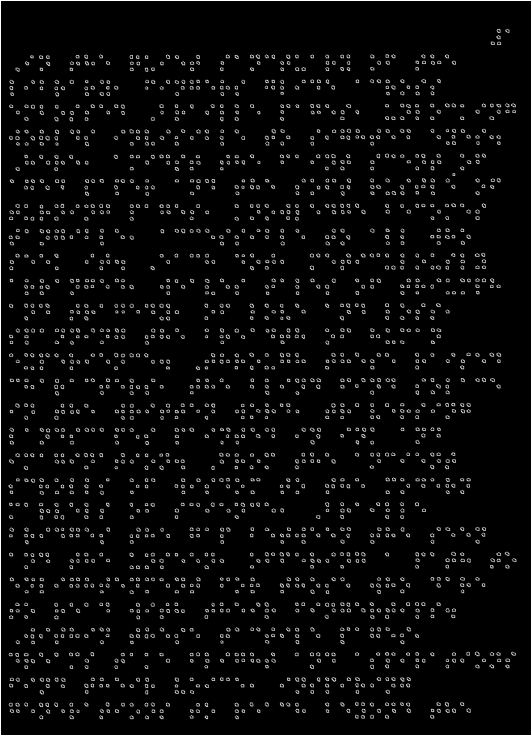
\includegraphics[width=0.5\linewidth]{Canny/Edges.png}}\\
    \caption{Canny Process Applied to the filtered \& upright Braille page}
    \label{fig:num2}
\end{figure}




\subsubsection{Circle Detection with Hough Transform}

\textbf{\textit{Theory of Hough Circle Transform}}

The Hough Circle Transform is a feature extraction technique used in image processing for detecting circles in an image. This method is an extension of the Hough Transform, which is widely used for detecting various shapes, especially lines. The classical Hough Transform for line detection involves mapping points from the image space to the parameter space, where lines in the image space correspond to points in the parameter space. Similarly, in the Hough Circle Transform, the goal is to identify circular shapes by mapping image space coordinates to the parameter space defined by the circle's parameters: center coordinates \((x_{center}, y_{center})\) and radius \(r\).

Mathematically, a circle can be described by the equation:
\begin{equation}
(x - x_{center})^2 + (y - y_{center})^2 = r^2
\end{equation}

where \((x_{center}, y_{center})\) represents the center of the circle and \(r\) its radius. To detect circles, the algorithm uses a parameter space that is three-dimensional, with dimensions corresponding to the circle's center coordinates and radius. For each edge point \((x, y)\) in the image, the possible circles passing through that point are determined, and an accumulator array in the parameter space is incremented accordingly. The peaks in this accumulator array indicate the parameters of the circles present in the image.

\textbf{\textit{Differences from Hough Gradient Method}}

The Hough Gradient Method, also known as the Hough Gradient Transform, is a more efficient variant of the classical Hough Circle Transform specifically designed for circle detection. While the traditional Hough Circle Transform involves a computationally expensive three-dimensional search for circle parameters, the Hough Gradient Method incorporates edge detection and gradient information to streamline this process.

The Hough Gradient Method reduces the computational complexity by taking advantage of the gradients of edge points. Here’s how it works:
\begin{enumerate}
        \item \textbf{Edge Detection:} Initially, an edge detection algorithm like Canny Edge Detector - discussed in section 5.1.1 - is applied to the image to find the edge points.
        \item \textbf{Gradient Computation:} For each edge point, the gradient direction is computed. The gradient direction indicates the direction of the center of the circle for that edge point.
        \item \textbf{Voting in Accumulator Space:} Using the gradient information, the algorithm only votes for circle centers along the gradient direction, significantly reducing the number of potential centers compared to the traditional method that votes in all directions.
\end{enumerate}


This method significantly enhances efficiency because it narrows down the potential circle centers by leveraging the directional information from gradients. Consequently, the Hough Gradient Method requires fewer computational resources and provides more accurate circle detection by reducing false positives.

Applying the Hough Gradient Method to the Braille page that has gone through the process of edge detection not only required low computational power, but also showed great results as it successfully detected all of the dots locations in the page. Figure \ref{fig:num3}(a) illustrates the detected dots whereas figure \ref{fig:num3}(b) shows a sample of how the raw output data looks like. This raw data of the dots locations is saved in an \textit{N-sized} array, we will call it later as \textbf{"Dots Locations Array"}, with each element representing the \((x_{center}, y_{center})_i\) of every Braille dot, where \textit{N} is the number of dots in a single Braille page, \textit{i} varies from \textit{1} to \textit{N}.



\begin{figure}[H]
    \centering
    \subfloat[Braille page after detecting dots using Hough Gradient]{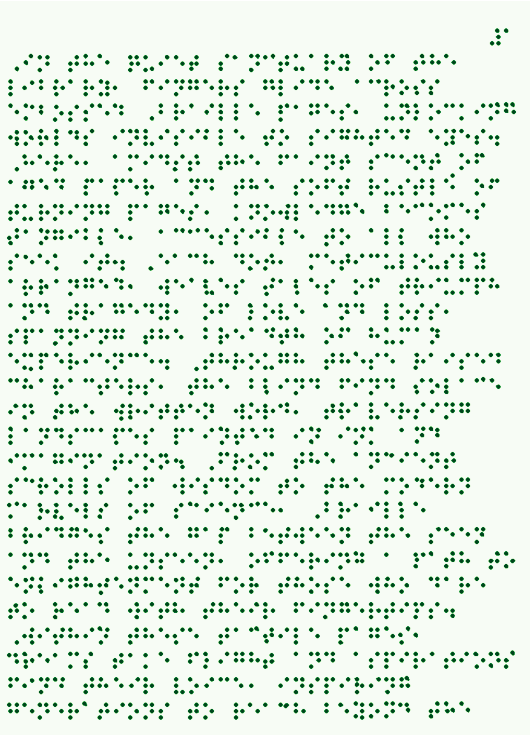
\includegraphics[width=0.55\linewidth]{Hough/Hough.png}}\hfill
    \subfloat[Some of the detected coordinates]{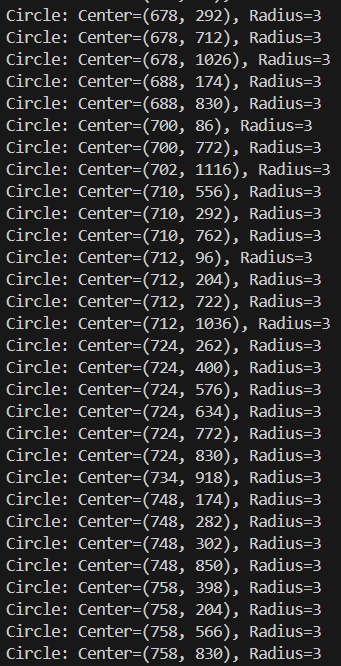
\includegraphics[width=0.39\linewidth]{Hough/snippent.png}}\\
    \caption{Hough Gradient Applied to the edge-detected Braille page}
    \label{fig:num3}
\end{figure}

\subsubsection{Identifying Braille Symbols}
In this section, we will cover the methods used to categorize dot locations stored in the Dots Locations Array. This involves several steps:
1. Sorting the Dots Locations Array: Sorted in ascending order based on X-coordinates.
2. Identifying all unique X-coordinate and Y-coordinate values containing potential dots: To mitigate potential shifts in dot centers, in cases where two unique X-coordinates or Y-coordinates closely align within a specified threshold, the higher X-coordinates or Y-coordinates are excluded, and \textbf{the corresponding dots are aligned with the lower coordinate values}, as shown in figure \ref{fig:num4}. These aligned dots locations are saved in an array that will be mentioned later as \textbf{"Aligned Locations Array"}.

\begin{figure}[H]
    \centering
    \subfloat[Before Alignment]{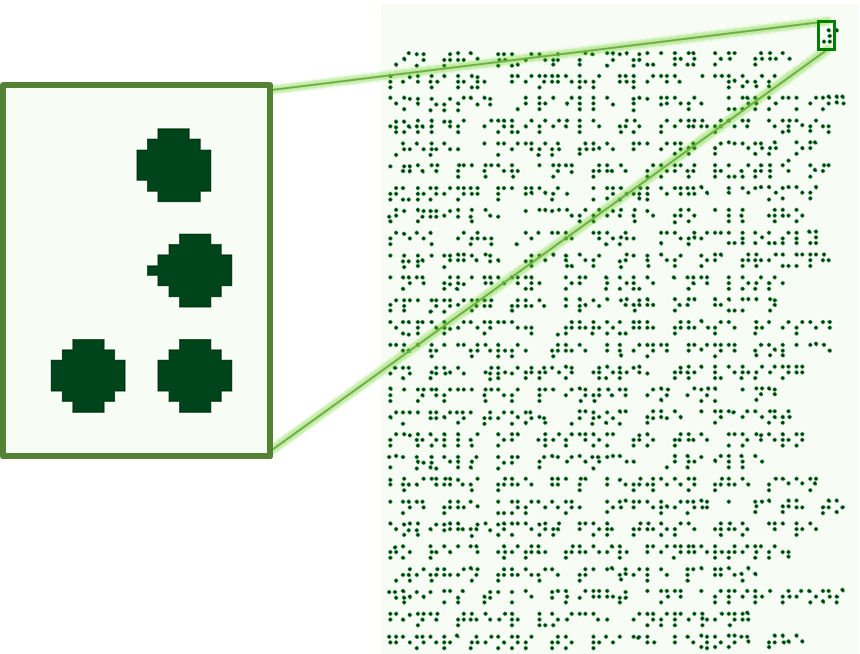
\includegraphics[width=1\linewidth]{Hough/Notalligned.png}}\\
    \subfloat[After Alignment]{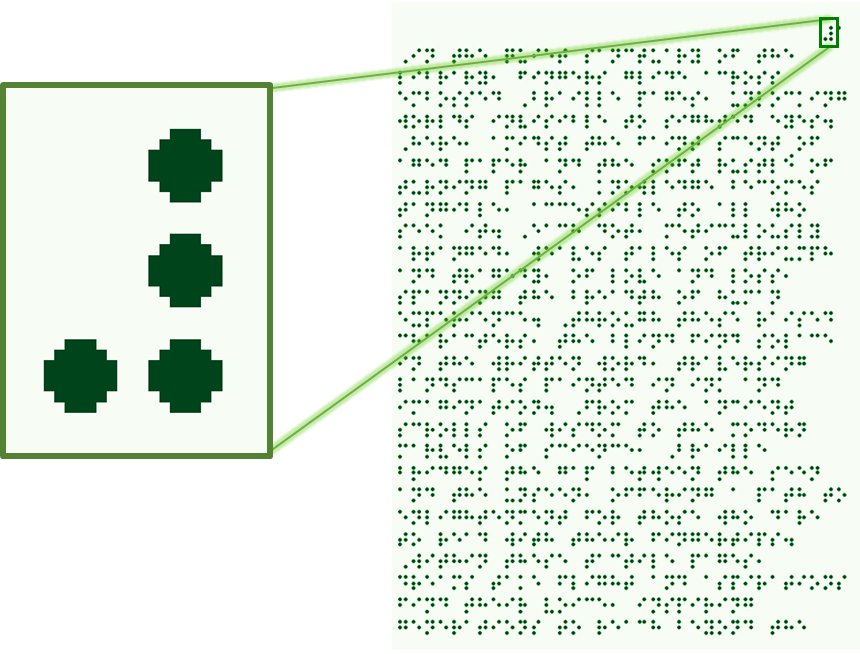
\includegraphics[width=1\linewidth]{Hough/Alligned.png}}\\
    \caption{Alignment Applied to the Braille Page.}
    \label{fig:num4}
\end{figure}


\subsubsection{A Challenge: Eliminating Unnecessary Extra Points}

One of the challenges we faced during the process was dealing with Braille Special Characters. These characters are composed of 8 dots instead of 6, and they are not globally used in formal Braille language. However, some of the Braille language users tend to abstract some of their frequently used words, signs, or expressions into one of these 8 dots symbols. Figure \ref{fig:num7} illustrates an example of an 8 dots special Braille symbol.

\begin{figure}[H]
    \centering
    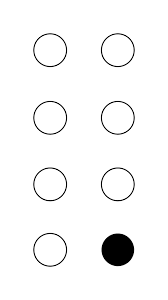
\includegraphics[width=0.25\linewidth]{Hough/8dots.png}
    \caption{8 dots special Braille symbol}
    \label{fig:num7}
\end{figure}

A couple of the sample pages we worked on while building our project had one of these special symbols, as shown in figure 5.6. As these symbols are not globally used and depend on user-based mapping, we decided to ignore the extra dot at any of the very bottom positions and deal with the character as a 6 dots normal symbol. This will definitely result in an incorrect character, but it will be probably corrected in the text correction stage (will be discussed in chapter 7).

\begin{figure}[H]
    \centering
    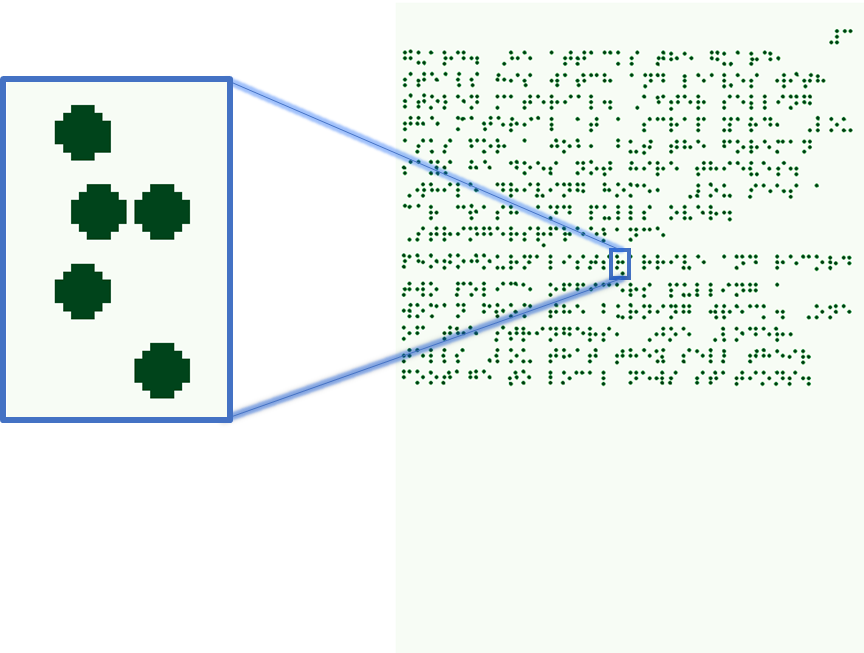
\includegraphics[width=0.85\linewidth]{Hough/Extra dot.png}
    \caption{8 dots special Braille symbol in on of the sample pages}
    \label{fig:num8}
\end{figure}


\subsection{Recognition}
In this section, we will cover the methods used to convert dot coordinates for each symbol into a binary combination of 6 dots. This process consists of 2 steps: Predicting Potential Dot Locations, and Mapping Braille Symbols into Binary. In the following subsections we will discuss the details of each step.

\subsubsection{Predicting Potential Dot Locations}
In this subsection, we will explain how the potential dot locations were predicted based on the detected dot locations. Following the alignment discussed in section 5.1.3, the program utilizes all unique X-coordinates and Y-coordinates to construct a matrix, where each element represents a potential dot space. The matrix elements are structured such that groups of six elements correspond to individual characters. These predictions are based on the aligned dot coordinates array.

To deliver the idea in a simpler way, assume each dot can be represented with an X-axis and a Y-axis passing through its center. Applying this assumption to all of the dots, \textbf{A virtual grid} is created as illustrated in figure \ref{fig:num5}(a). Red dots represent potential dots locations. \textbf{RED DOTS ARE JUST FOR ILLUSTRATION, THEY ARE NOT A PART OF THE ORIGINAL PAGE.} At each and every intersection, there should be a potential dot location. Based on this concept, a matrix is created, called \textbf{"General Matrix"}, including all of the potential dots locations. This means that the matrix size is MxN where M is the number of symbols rows and N is the number of symbols columns. Each element in the matrix has a size of 1x6, as there are 6 potential dots for each symbol. Figure \ref{fig:num5}(b) represents the potential dots locations in the first row of the page as a sample of the matrix. Figure \ref{fig:num9} illustrates all of the potential dots locations saved in General Matrix.

\begin{figure}[H]
    \begin{adjustwidth}{-2.5cm}{}
        \centering
        \subfloat[Virtual Grid Based on Aligned Dot Coordinates array]{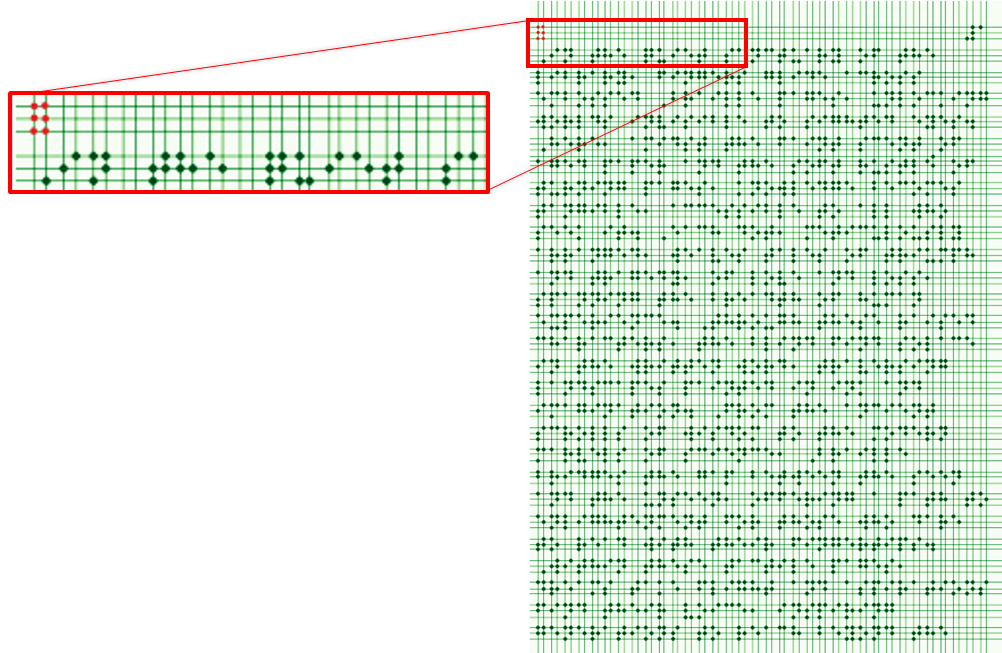
\includegraphics[width=1.1\linewidth]{Hough/Grid.png}}\\
        \subfloat[Potential dots locations in the 1st row in the page]{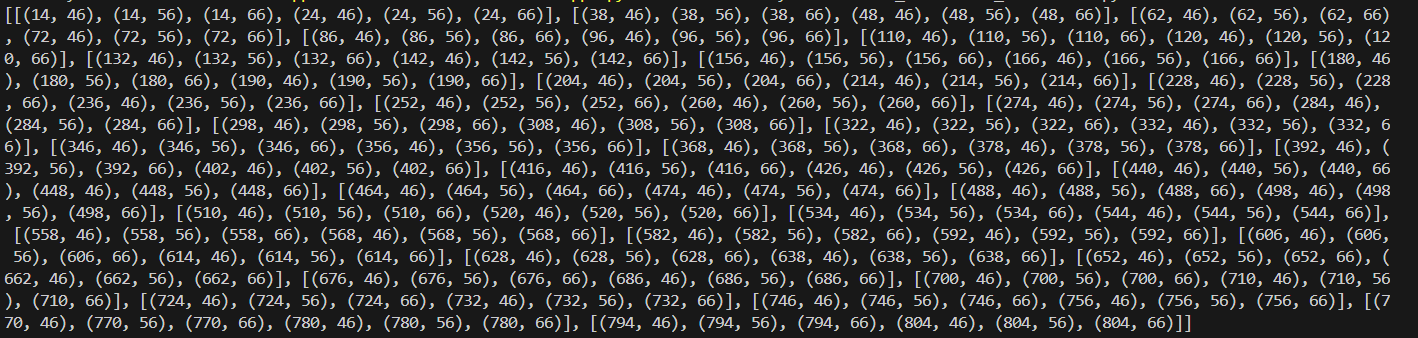
\includegraphics[width=1.1\linewidth]{Hough/image.png}}\\
    \end{adjustwidth}
    \caption{Potential Dots Prediction}
    \label{fig:num5}
\end{figure}

Currently, it should be clear enough why we assumed that the page should be full of symbols at the very beginning of this chapter. It is because the accuracy of predicting all of the potential dots locations is directly proportional to number of symbols present in a single Braille page. This means, for a page that barely contains symbols, the virtual grid wouldn't fully form. Therefore, the General Matrix wouldn't be fully filled and the recognition process would lack accuracy.
\begin{figure}[H]
    \centering
    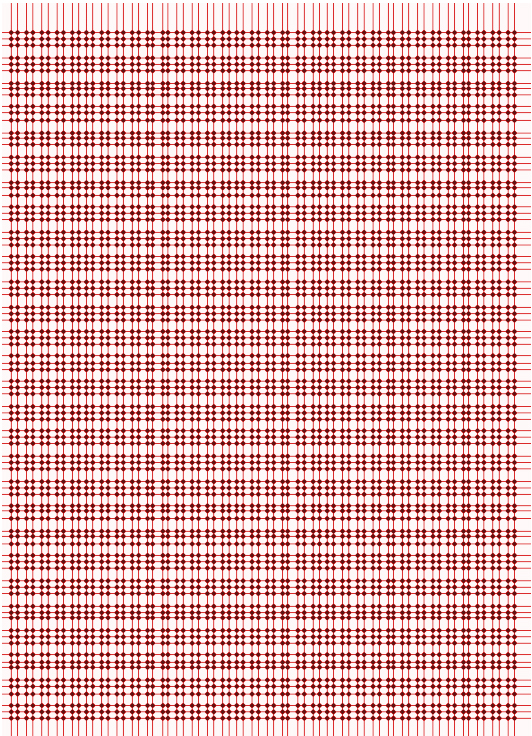
\includegraphics[width=0.8\linewidth]{Hough/red.jpg}
    \caption{All of the potential dots locations saved in General Matrix}
    \label{fig:num9}
\end{figure}

\subsubsection{Identifying Braille Symbols and Mapping Braille Symbols into Binary}

The next step is to identify Braille symbols. In order to do this, We're masking the Aligned Locations Array mentioned in section 5.1.3 on the General Matrix mentioned in the previous section. The masking process is illustrated in figure \ref{fig:num8}.  All of the red dots overlapping with green dots represent 1s, while all of the red dots overlapping with empty spaces represent 0s. With the fact that the General Matrix is already symbolized, The Aligned locations array is going to be symbolized and binary mapped after masking into a new array named \textbf{"Updated Symbols"}. Updated symbols array contains multiple rows, where each row contains multiple symbols, where each symbols contains 6 binary values, where ones represent that there is a present dot and zeros represent that there is no dot. Figure \ref{fig:num6} shows the first element of the Updated Symbols array, which represents the first row of the page after being symbolized and mapped to binary.

\begin{figure}[H]
    \begin{adjustwidth}{-1.5cm}{}
      \centering
      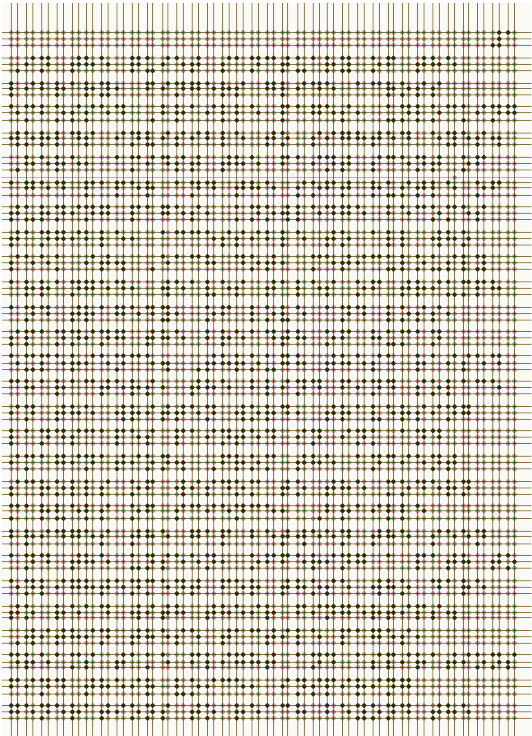
\includegraphics[width=1.12\linewidth]{Hough/mask.jpg}
    \end{adjustwidth}
    \caption{Masking Process}
    \label{fig:num8}
\end{figure}

\begin{figure}[H]
    \begin{adjustwidth}{-2.5cm}{}
        \centering
        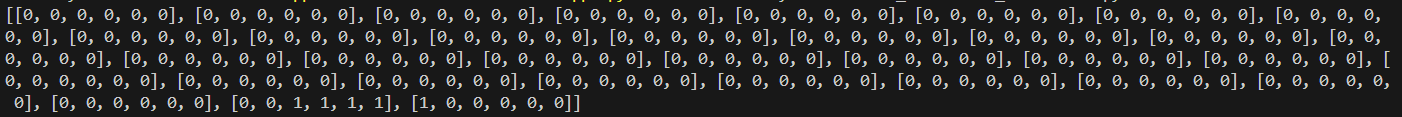
\includegraphics[width=1.12\linewidth]{Hough/image1.png}
    \end{adjustwidth}
    \caption{1st row of the page after being symbolized and mapped to binary}
    \label{fig:num6}
\end{figure}

The next key step is to simply to translate every symbol into its corresponding alphabetic letter. This step will be discussed in detail later in chapter 7 .